\section{WhyCode Modifications}
\label{section:whycode_modifications}

The WhyCon fiducial marker, shown in Figure \ref{fig:whycon} consists of a white circle inside of a larger black circle.
The identification algorithm is computationally simple:
\begin{itemize}
    \item A rectified image is searched for white regions.
    \item The detector flood-fills and determines a measure of circularity for each white region.
    \item The detector seeks a black region directly outside of each white region, flood fills it, and determines a measure of circularity for it.
    \item The circularity measures are compared, and the white/black region combination is called a WhyCon marker if it is adequately circular (under projection).
    \item The major and minor axes provide a basis from which to determine the marker's orientation.
    \item The position of the marker is determined using the pinhole model of a monocular camera with known intrinsic parameters
            (pixel resolution, lens distortion, principal points, focal lengths), and the diameter of the marker.
\end{itemize}

The WhyCon system's purpose is to determine the pose (position \textit{and} orientation) of detected WhyCon markers.
The position of the markers is

\begin{figure}[h]
    \centering
    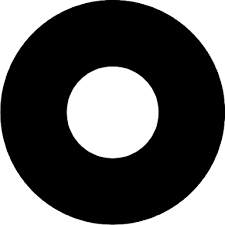
\includegraphics[width=0.16\textwidth]{images/whycon_example.png}
    \caption{WhyCon marker.}
    \label{fig:whycon}
\end{figure}

\begin{figure}[h]
    \centering
    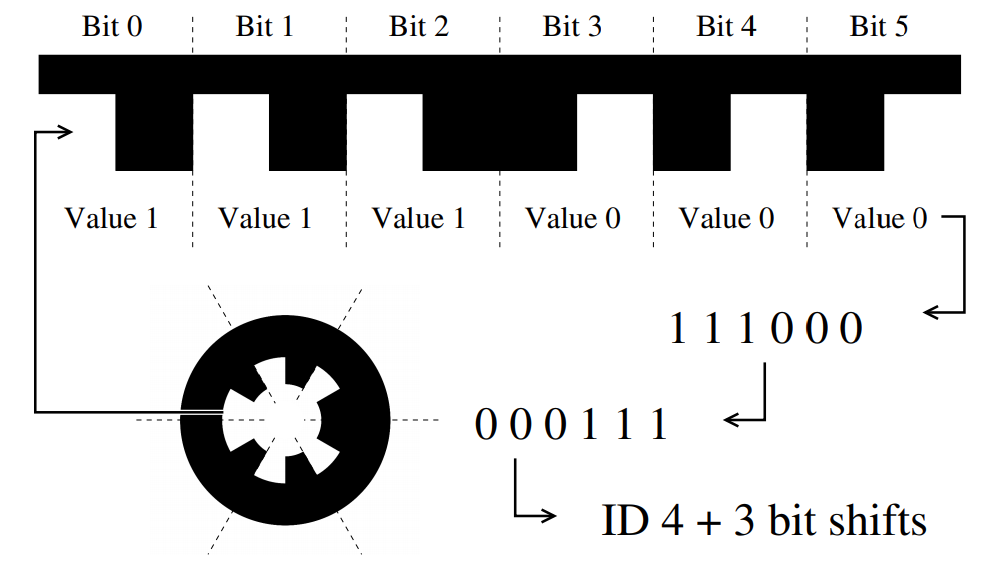
\includegraphics[width=0.4\textwidth]{images/whycode_manchester_explanation.png}
    \caption{WhyCode ID Manchester ``Necklace'' Encoding.}
    \label{fig:whycode_id}
\end{figure}

\begin{figure}[h]
    \centering
    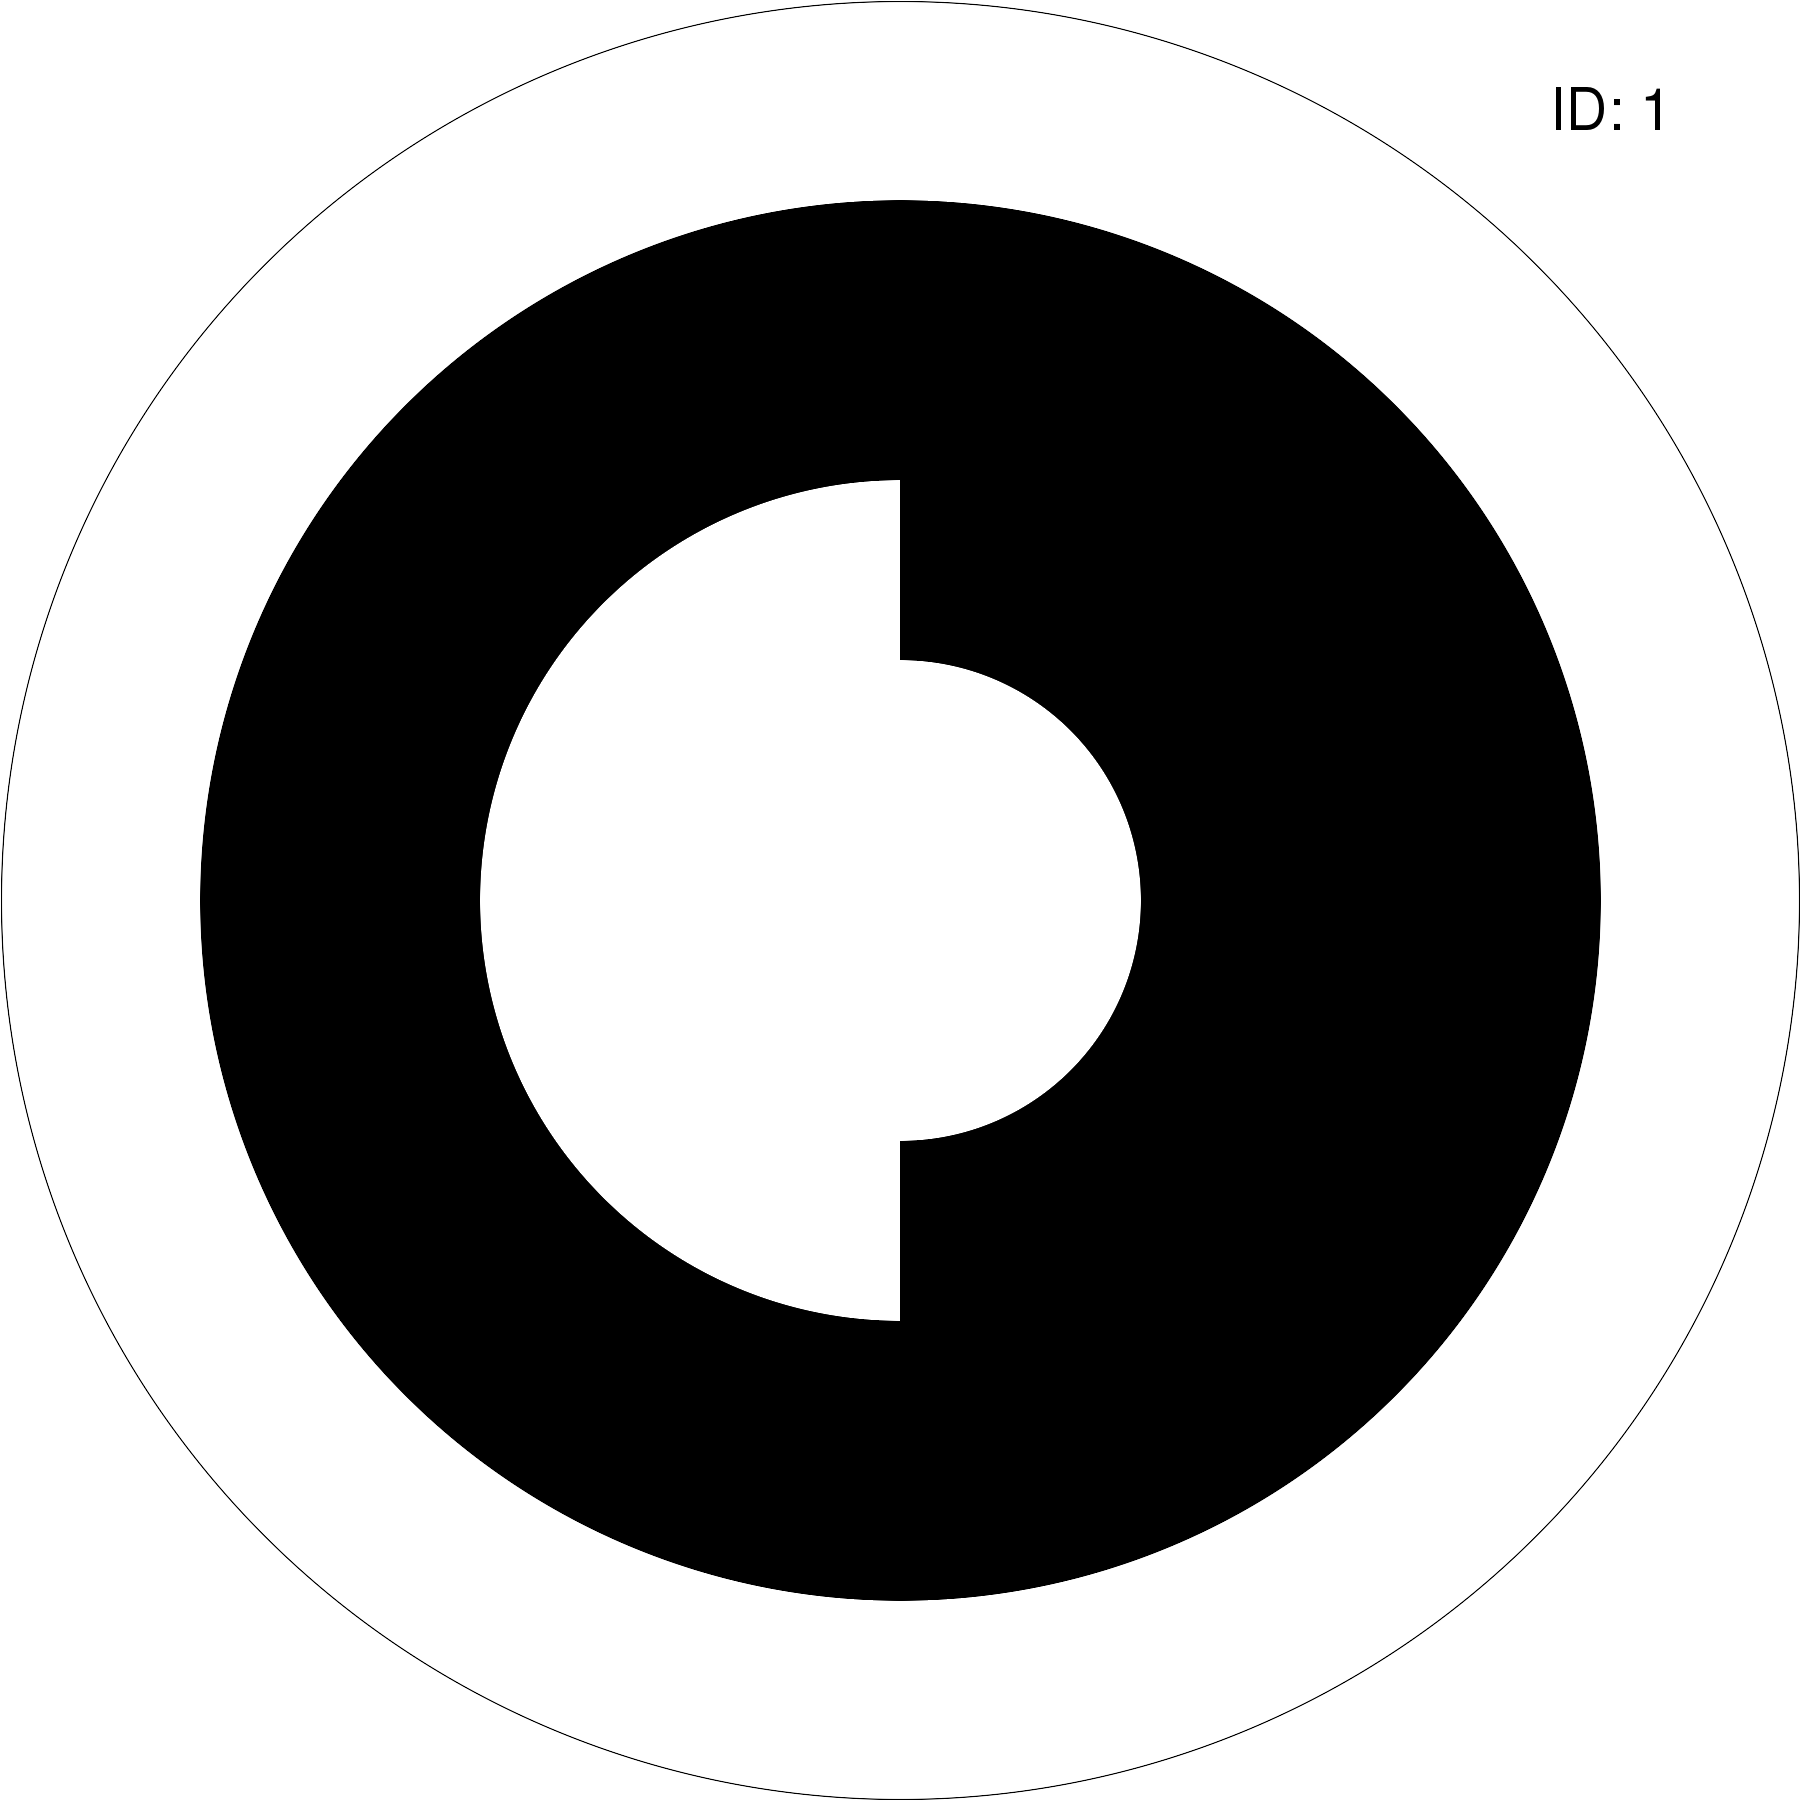
\includegraphics[width=0.2\textwidth]{images/00000001.png}
    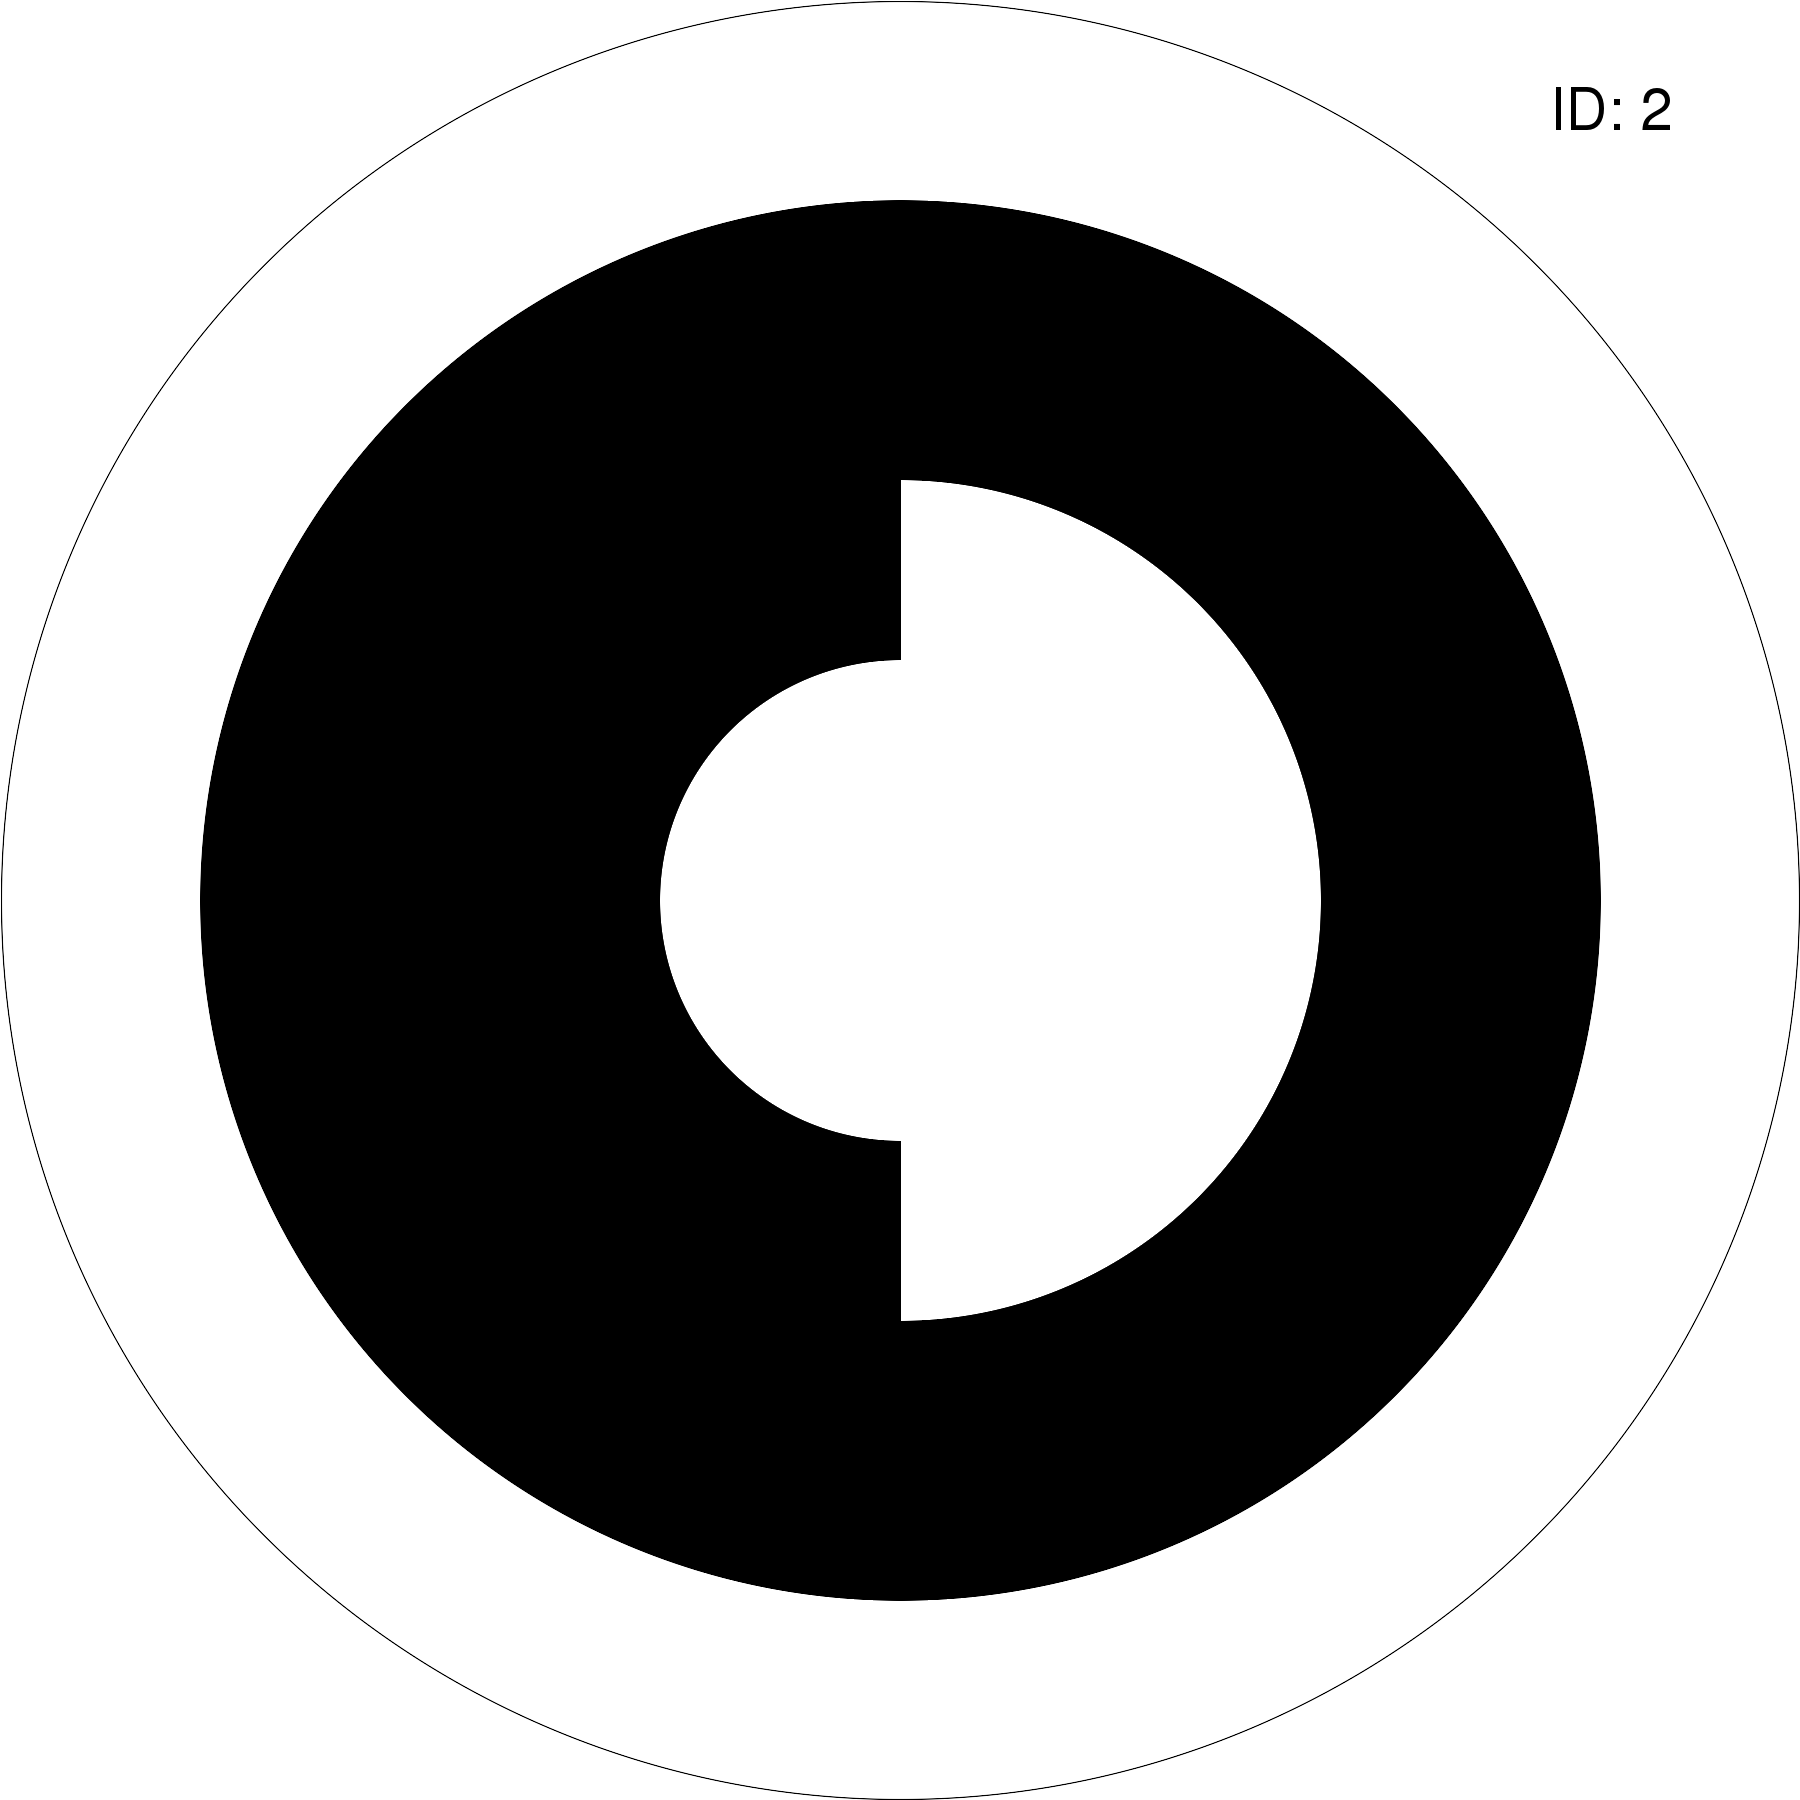
\includegraphics[width=0.2\textwidth]{images/00000002.png}
    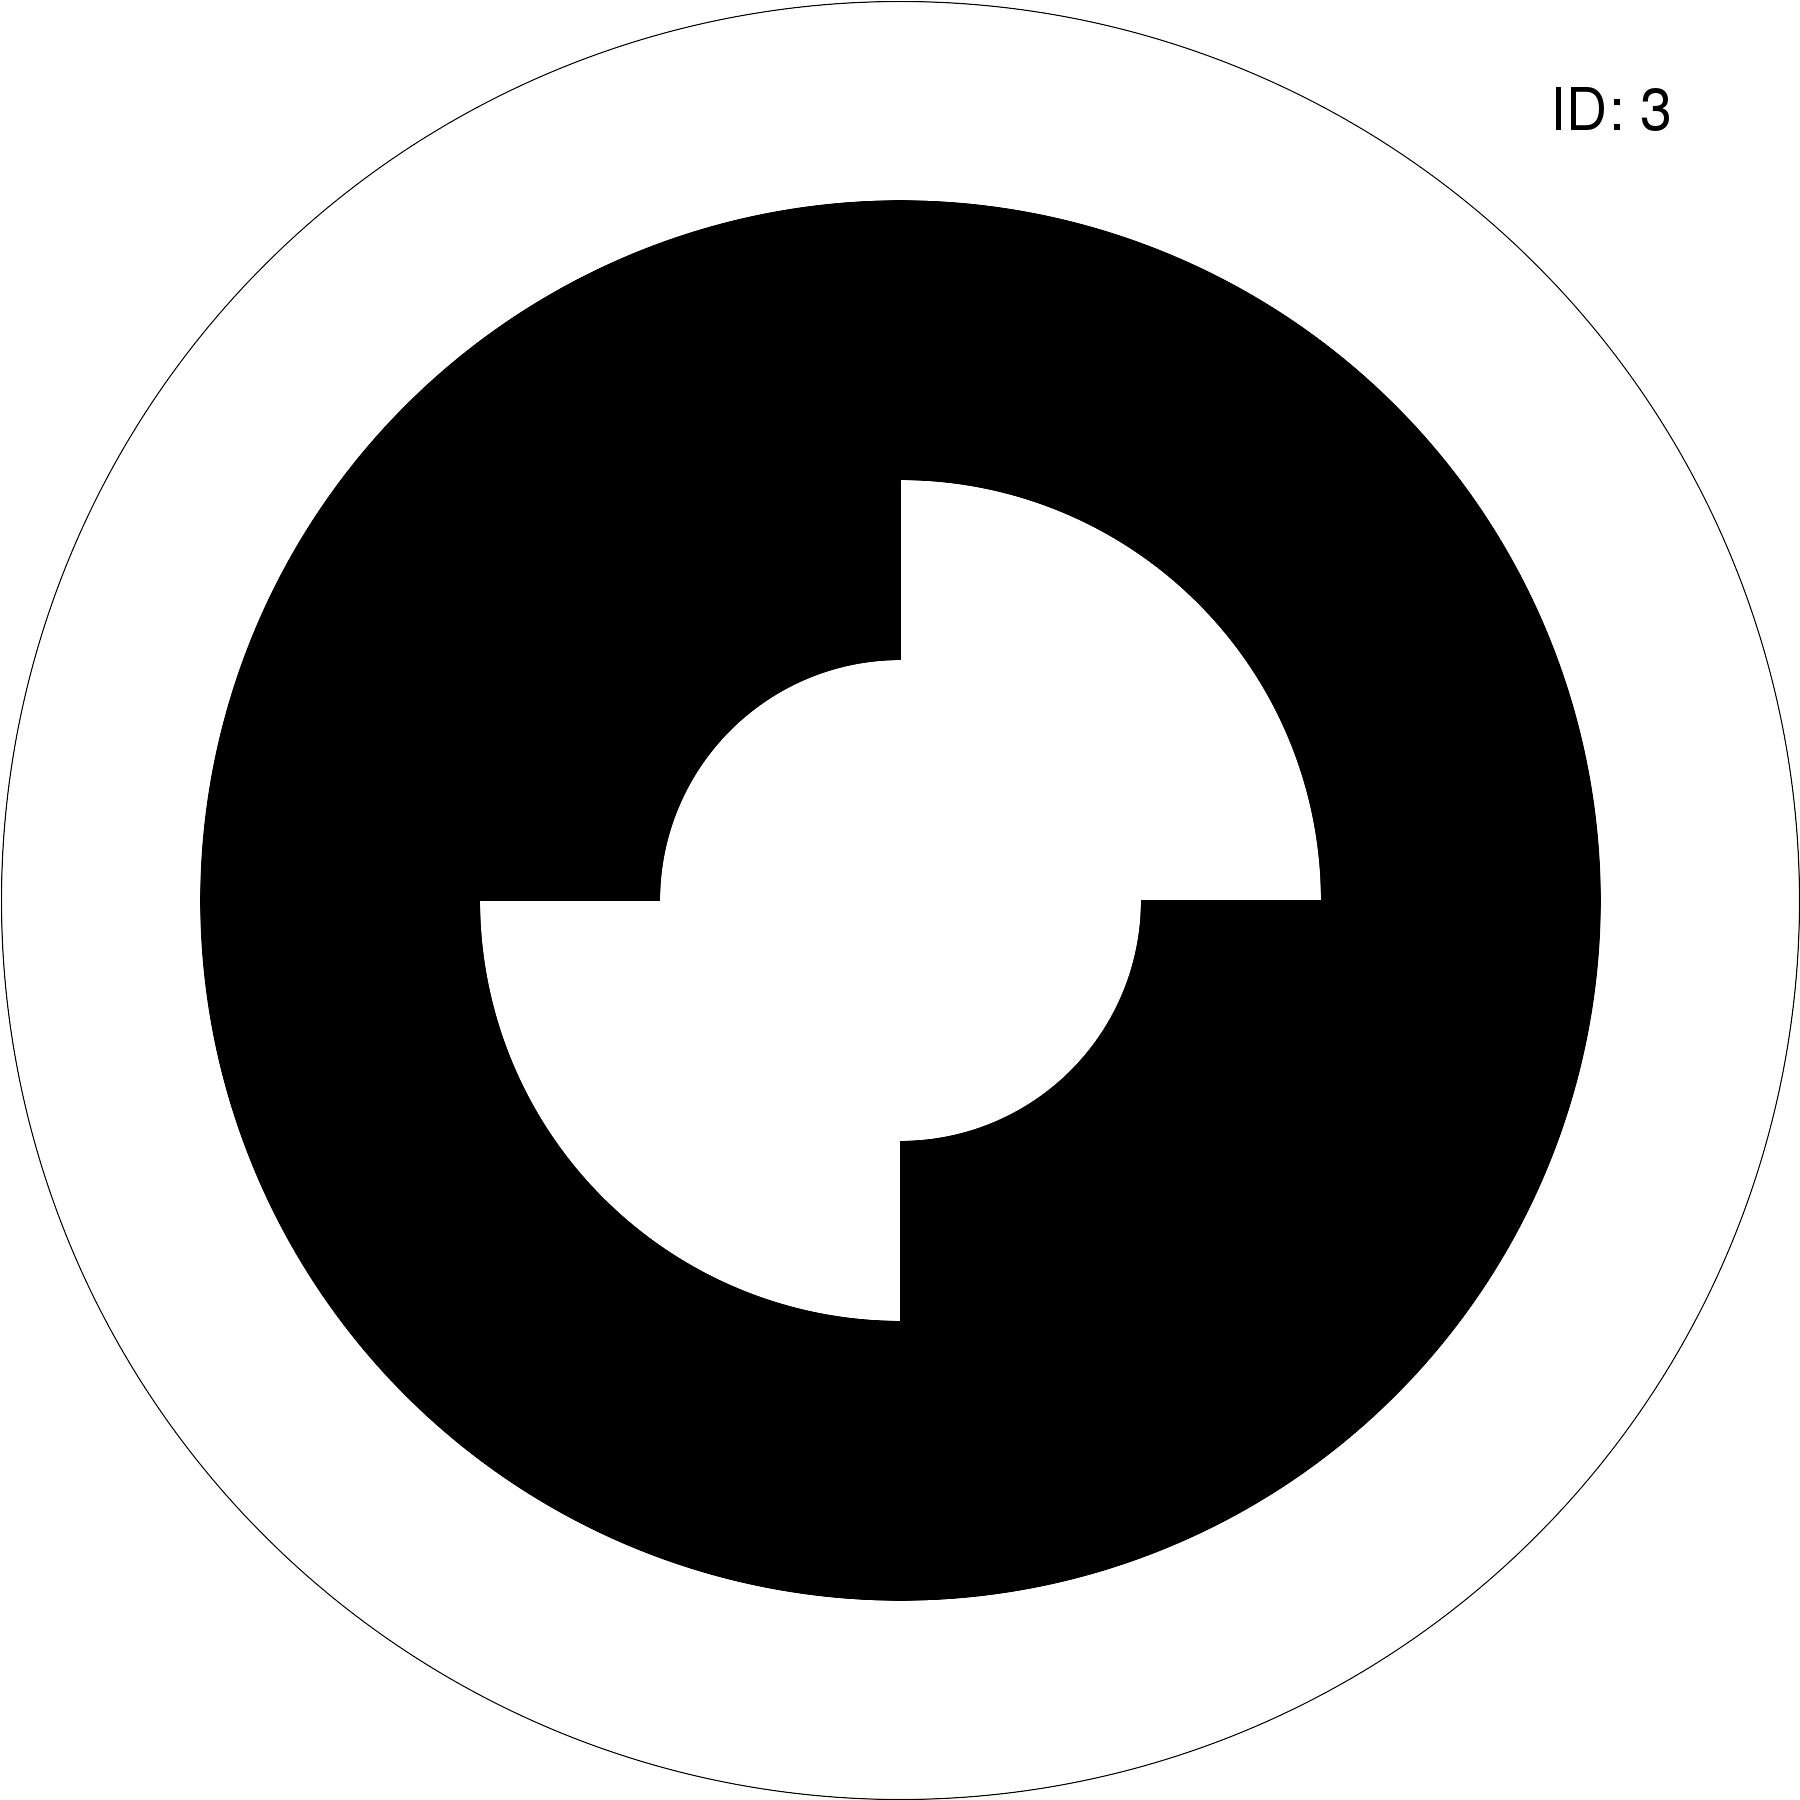
\includegraphics[width=0.2\textwidth]{images/00000003.png}
    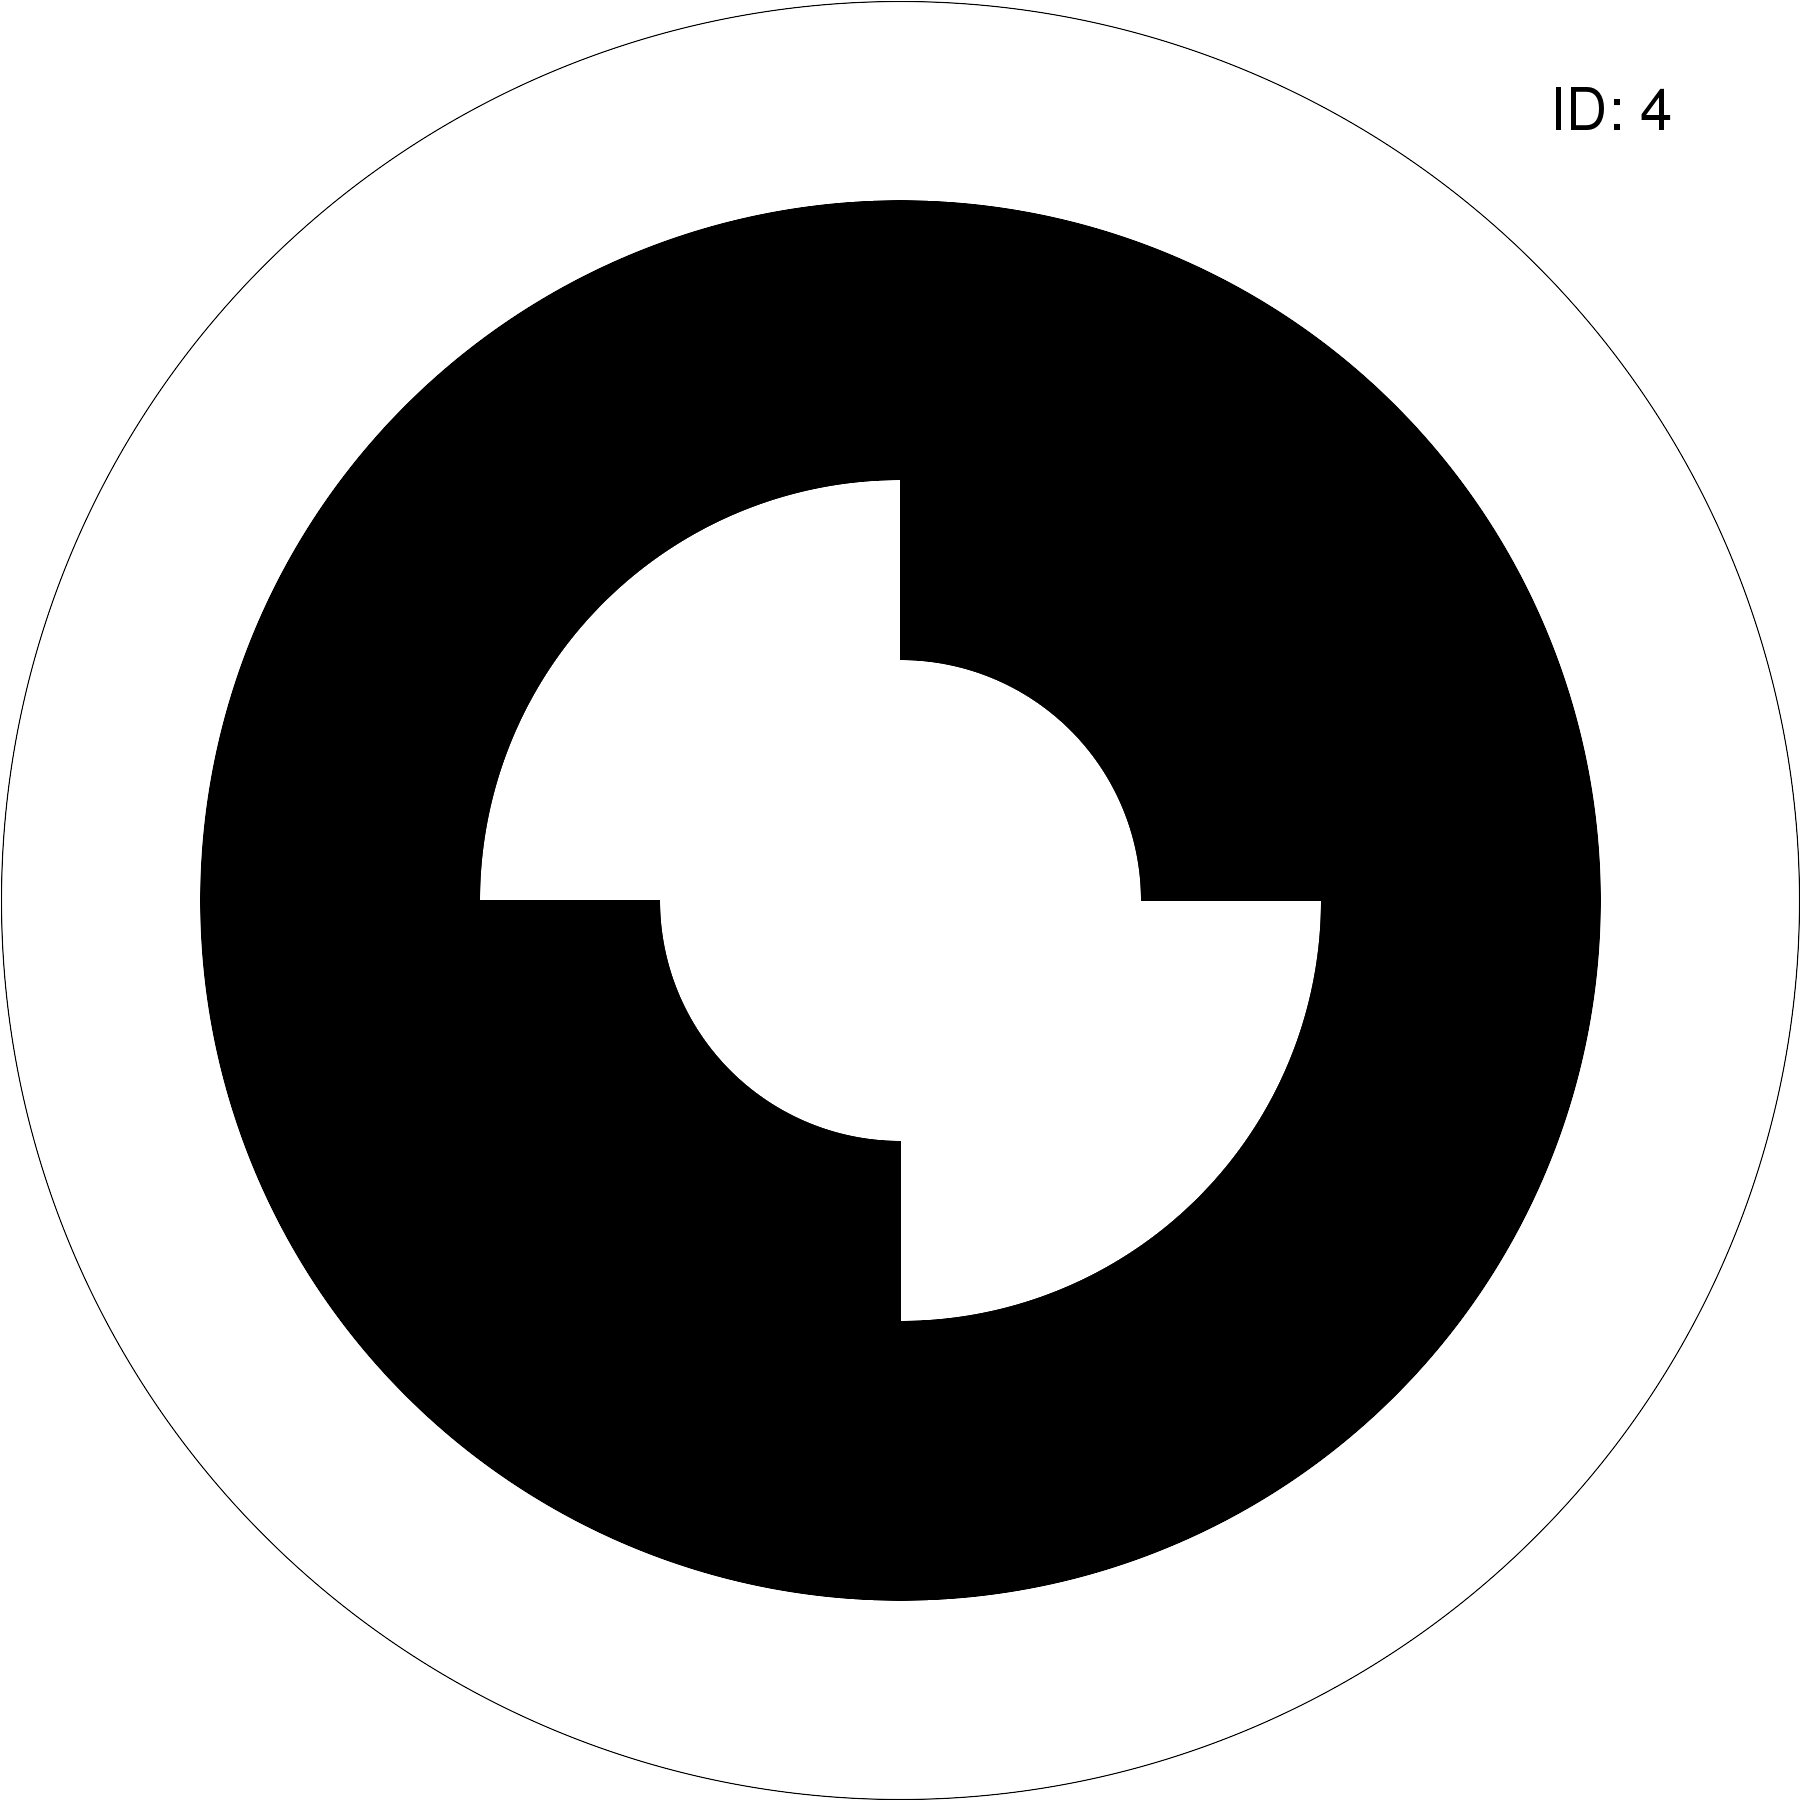
\includegraphics[width=0.2\textwidth]{images/00000004.png}
    \caption{Rotational symmetry in 2-bit WhyCode markers.}
    \label{fig:rotationally_symmetric_whycode_markers}
\end{figure}